\documentclass[12pt,aspectratio=169]{beamer}

% ── Tema ──────────────────────────────────────────────────────────
\usetheme{Madrid}
\usecolortheme{seahorse}

\definecolor{azul}{RGB}{10,60,120}
\definecolor{azulm}{RGB}{30,100,180}
\definecolor{dorado}{RGB}{180,130,0}
\definecolor{verde}{RGB}{0,130,90}
\definecolor{gris}{RGB}{245,245,250}

\setbeamercolor{palette primary}{bg=azul,fg=white}
\setbeamercolor{palette secondary}{bg=azulm,fg=white}
\setbeamercolor{palette tertiary}{bg=dorado,fg=white}
\setbeamercolor{palette quaternary}{bg=azul,fg=white}
\setbeamercolor{structure}{fg=azul}
\setbeamercolor{frametitle}{bg=azul,fg=white}
\setbeamercolor{block title}{bg=azul,fg=white}
\setbeamercolor{block body}{bg=gris,fg=black}
\setbeamercolor{block title alerted}{bg=dorado,fg=white}
\setbeamercolor{block body alerted}{bg=dorado!15,fg=black}
\setbeamercolor{block title example}{bg=verde,fg=white}
\setbeamercolor{block body example}{bg=verde!12,fg=black}

% ── Paquetes ──────────────────────────────────────────────────────
\usepackage[T1]{fontenc}
\usepackage[utf8]{inputenc}
\usepackage{amsmath,amssymb,mathtools}
\usepackage{array,booktabs,tabularx}
\usepackage{tikz}
\usetikzlibrary{arrows.meta,shapes,positioning,calc,decorations.pathreplacing}
\usepackage{pgfplots}
\pgfplotsset{compat=1.18}
\usepackage{tcolorbox}
\tcbuselibrary{theorems,skins}
\usepackage{multicol}
\usepackage{pifont}

% ── Cajas ─────────────────────────────────────────────────────────
\newtcolorbox{cdef}[1]{
  enhanced,title=#1,colback=azul!6,colframe=azul,
  fonttitle=\bfseries\small,coltitle=white,
  attach boxed title to top left={yshift=-2mm,xshift=4mm},
  boxed title style={colback=azul},top=5pt,left=5pt,right=5pt,bottom=5pt
}
\newtcolorbox{cprop}[1]{
  enhanced,title=#1,colback=azulm!8,colframe=azulm,
  fonttitle=\bfseries\small,coltitle=white,
  attach boxed title to top left={yshift=-2mm,xshift=4mm},
  boxed title style={colback=azulm},top=5pt,left=5pt,right=5pt,bottom=5pt
}
\newtcolorbox{cejec}[1]{
  enhanced,title=\ding{46}\;#1,colback=verde!8,colframe=verde,
  fonttitle=\bfseries\small,coltitle=white,
  attach boxed title to top left={yshift=-2mm,xshift=4mm},
  boxed title style={colback=verde},top=5pt,left=5pt,right=5pt,bottom=5pt
}
\newtcolorbox{calert}[1]{
  enhanced,title=\ding{72}\;#1,colback=dorado!12,colframe=dorado,
  fonttitle=\bfseries\small,coltitle=white,
  attach boxed title to top left={yshift=-2mm,xshift=4mm},
  boxed title style={colback=dorado},top=5pt,left=5pt,right=5pt,bottom=5pt
}

% ── Pie de pagina ─────────────────────────────────────────────────
\setbeamertemplate{navigation symbols}{}
\setbeamertemplate{footline}{
  \leavevmode\hbox{%
    \begin{beamercolorbox}[wd=.33\paperwidth,ht=2.4ex,dp=1ex,leftskip=3mm]{palette primary}
      \usebeamerfont{author in head/foot}\insertshortauthor
    \end{beamercolorbox}%
    \begin{beamercolorbox}[wd=.34\paperwidth,ht=2.4ex,dp=1ex,center]{palette secondary}
      \usebeamerfont{title in head/foot}\insertshorttitle
    \end{beamercolorbox}%
    \begin{beamercolorbox}[wd=.33\paperwidth,ht=2.4ex,dp=1ex,rightskip=3mm,right]{palette primary}
      \insertframenumber{}/\inserttotalframenumber
    \end{beamercolorbox}}\vskip0pt}

% ── Metadatos ─────────────────────────────────────────────────────
\title[Potencias y \'{A}lgebra Real]{\textbf{Potencias y \'{A}lgebra en los N\'{u}meros Reales}}
\subtitle{Fundamentos, Propiedades y Patrones Algebraicos}
\author[Matem\'{a}ticas]{C\'{a}tedra de Matem\'{a}ticas}
\institute[Universidad]{Departamento de Ciencias Exactas\\[2pt]
  \small C\'{a}lculo y \'{A}lgebra -- Primer Semestre}
\date{\today}

% ══════════════════════════════════════════════════════════════════
\begin{document}
% ══════════════════════════════════════════════════════════════════

% ── PORTADA ───────────────────────────────────────────────────────
{
\setbeamertemplate{headline}{}
\setbeamertemplate{footline}{}
\begin{frame}
  \begin{tikzpicture}[remember picture,overlay]
    \fill[azul] (current page.north west)
      rectangle ([yshift=-0.36\paperheight]current page.north east);
    \fill[dorado] ([yshift=-0.36\paperheight]current page.north west)
      rectangle ([yshift=-0.39\paperheight]current page.north east);
    \node[anchor=north,text=white,font=\Large\bfseries]
      at ([yshift=-1.1cm]current page.north)
      {POTENCIAS Y \'ALGEBRA EN LOS N\'UMEROS REALES};
    \node[anchor=north,text=dorado!60!white,font=\normalsize\itshape]
      at ([yshift=-2.3cm]current page.north)
      {Fundamentos, Propiedades y Patrones Algebraicos};
  \end{tikzpicture}
  \vspace*{4.2cm}
  \begin{columns}[T]
    \column{0.52\textwidth}
    {\color{azul}\textbf{\large Contenidos:}}\\[5pt]
    \small
    \begin{itemize}
      \item[\textcolor{dorado}{$\blacktriangleright$}] Concepto y propiedades de potencias
      \item[\textcolor{dorado}{$\blacktriangleright$}] T\'erminos y expresiones algebraicas
      \item[\textcolor{dorado}{$\blacktriangleright$}] T\'erminos semejantes y simplificaci\'on
      \item[\textcolor{dorado}{$\blacktriangleright$}] Patrones y relaciones algebraicas
    \end{itemize}
    \column{0.42\textwidth}
    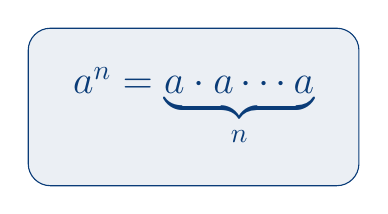
\begin{tikzpicture}
      \node[draw=azul,fill=azul!8,rounded corners=8pt,
            minimum width=4.2cm,minimum height=2cm,
            font=\Large\bfseries,text=azul] at (0,0)
            {$a^n = \underbrace{a \cdot a \cdots a}_{n}$};
    \end{tikzpicture}
  \end{columns}
\end{frame}
}

% ── INDICE ────────────────────────────────────────────────────────
\begin{frame}{\'{I}ndice}
  \begin{columns}
    \column{0.5\textwidth}\tableofcontents[sections={1-2}]
    \column{0.5\textwidth}\tableofcontents[sections={3-4}]
  \end{columns}
\end{frame}

% ══════════════════════════════════════════════════════════════════
\section{Concepto de Potencia}
% ══════════════════════════════════════════════════════════════════

\begin{frame}{?`Qu\'{e} es una Potencia?}
  \begin{columns}[T]
    \column{0.52\textwidth}
    \begin{cdef}{Definici\'on Formal}
      Sea $a\in\mathbb{R}$ y $n\in\mathbb{N}$. La \textbf{potencia} de base $a$
      y exponente $n$ es:
      \[
        a^n \;=\; \underbrace{a\cdot a\cdots a}_{n\text{ factores}},\quad n\ge 1
      \]
      Convenio: $a^{0}=1$ para $a\neq 0$.
    \end{cdef}
    \vspace{5pt}
    \begin{calert}{Caso especial: $0^0$}
      La expresi\'on $0^0$ es una \textbf{indeterminaci\'on} en an\'alisis.
      En combinatoria se adopta el convenio $0^0=1$.
    \end{calert}

    \column{0.44\textwidth}
    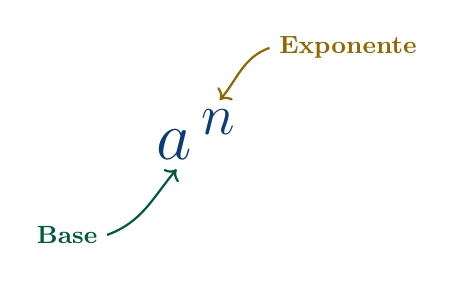
\begin{tikzpicture}
      \node[font=\Huge\bfseries,text=azul] (ex) at (0,0) {$a^{\,n}$};
      \node[font=\small,text=verde!70!black,
            below left=0.6cm and 0.5cm of ex] (b) {\textbf{Base}};
      \node[font=\small,text=dorado!80!black,
            above right=0.4cm and 0.3cm of ex] (e) {\textbf{Exponente}};
      \draw[->,verde!70!black,thick] (b.east) to[out=20,in=230]
        ([xshift=-0.25cm]ex.south);
      \draw[->,dorado!80!black,thick] (e.west) to[out=200,in=50]
        ([xshift=0.3cm]ex.north);
    \end{tikzpicture}
    \vspace{6pt}

    \renewcommand{\arraystretch}{1.35}
    \begin{tabular}{ccc}
      \toprule
      Potencia & Desarrollo & Valor\\
      \midrule
      $2^{4}$ & $2{\cdot}2{\cdot}2{\cdot}2$ & $16$\\
      $(-3)^{2}$ & $(-3)(-3)$ & $9$\\
      $5^{0}$ & (convenio) & $1$\\
      $\bigl(\tfrac{1}{2}\bigr)^{3}$ & $\tfrac{1}{2}{\cdot}\tfrac{1}{2}{\cdot}\tfrac{1}{2}$ & $\tfrac{1}{8}$\\
      \bottomrule
    \end{tabular}
  \end{columns}
\end{frame}

\begin{frame}{Exponentes Enteros Negativos}
  \begin{columns}[T]
    \column{0.48\textwidth}
    \begin{cdef}{Exponente negativo}
      Para $a\neq 0$ y $n\in\mathbb{N}$:
      \[a^{-n}=\dfrac{1}{a^{n}}\]
    \end{cdef}
    \vspace{5pt}
    \begin{block}{Patr\'on motivador}
      \medskip
      \renewcommand{\arraystretch}{1.4}
      \centering
      \begin{tabular}{cc}
        \toprule
        Potencia & Valor\\\midrule
        $2^{3}$ & $8$\\
        $2^{2}$ & $4$\\
        $2^{1}$ & $2$\\
        $2^{0}$ & $1$\\
        $2^{-1}$ & $1/2$\\
        $2^{-2}$ & $1/4$\\
        \bottomrule
      \end{tabular}
    \end{block}

    \column{0.48\textwidth}
    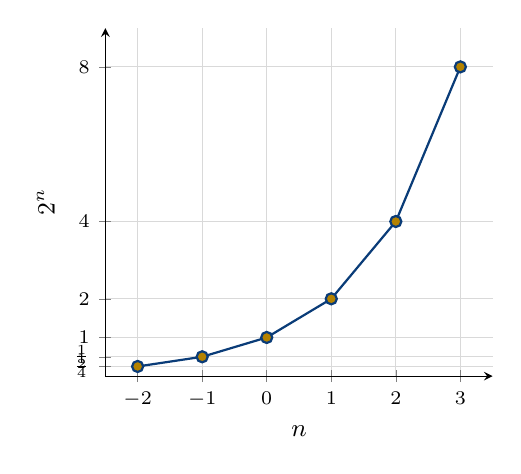
\begin{tikzpicture}
      \begin{axis}[
        width=6.5cm,height=6cm,
        xlabel={$n$},ylabel={$2^n$},
        xlabel style={font=\small},
        ylabel style={font=\small},
        xtick={-2,-1,0,1,2,3},
        ytick={0.25,0.5,1,2,4,8},
        yticklabels={$\frac14$,$\frac12$,$1$,$2$,$4$,$8$},
        tick label style={font=\scriptsize},
        grid=both,grid style={gray!30},
        axis lines=left,ymin=0,ymax=9,xmin=-2.5,xmax=3.5]
        \addplot[azul,thick,mark=*,mark options={fill=dorado,draw=azul}]
          coordinates{(-2,0.25)(-1,0.5)(0,1)(1,2)(2,4)(3,8)};
      \end{axis}
    \end{tikzpicture}
    \vspace{4pt}
    \begin{block}{$\star$ Patr\'on detectado}
      \small Cada vez que el exponente baja en $1$,
      el valor se \textbf{divide} entre la base.
      Este patr\'on \emph{define} los exponentes negativos.
    \end{block}
  \end{columns}
\end{frame}

% ══════════════════════════════════════════════════════════════════
\section{Propiedades de las Potencias}
% ══════════════════════════════════════════════════════════════════

\begin{frame}{Propiedades Fundamentales}
  \begin{columns}[T]
    \column{0.48\textwidth}
    \begin{cprop}{P1 $\cdot$ Producto (misma base)}
      $a^{m}\cdot a^{n}=a^{m+n}$\quad
      \textit{Ej.:} $x^{3}\cdot x^{5}=x^{8}$
    \end{cprop}\vspace{4pt}
    \begin{cprop}{P2 $\cdot$ Cociente (misma base)}
      $\dfrac{a^{m}}{a^{n}}=a^{m-n},\ a\neq0$\quad
      \textit{Ej.:} $\dfrac{y^{7}}{y^{3}}=y^{4}$
    \end{cprop}\vspace{4pt}
    \begin{cprop}{P3 $\cdot$ Potencia de potencia}
      $\bigl(a^{m}\bigr)^{n}=a^{mn}$\quad
      \textit{Ej.:} $\bigl(z^{2}\bigr)^{5}=z^{10}$
    \end{cprop}

    \column{0.48\textwidth}
    \begin{cprop}{P4 $\cdot$ Potencia de producto}
      $(ab)^{n}=a^{n}b^{n}$\quad
      \textit{Ej.:} $(2x)^{3}=8x^{3}$
    \end{cprop}\vspace{4pt}
    \begin{cprop}{P5 $\cdot$ Potencia de cociente}
      $\left(\dfrac{a}{b}\right)^{n}=\dfrac{a^{n}}{b^{n}},\ b\neq0$\quad
      \textit{Ej.:} $\left(\dfrac{x}{3}\right)^{2}=\dfrac{x^{2}}{9}$
    \end{cprop}\vspace{4pt}
    \begin{calert}{Errores frecuentes}
      \small
      $\bullet\ (a+b)^{2}\neq a^{2}+b^{2}$\\
      $\bullet\ a^{m}\cdot b^{n}\neq(ab)^{m+n}$ (bases distintas)
    \end{calert}
  \end{columns}
\end{frame}

\begin{frame}{Demostraci\'on de P1 y Aplicaci\'on}
  \begin{block}{Demostraci\'on: $a^{m}\cdot a^{n}=a^{m+n}$}
    \[
      a^{m}\cdot a^{n}
      =\underbrace{(a\cdots a)}_{m}\cdot\underbrace{(a\cdots a)}_{n}
      =\underbrace{a\cdots a}_{m+n}=a^{m+n}\qquad\square
    \]
  \end{block}
  \vspace{6pt}
  \begin{cejec}{Aplicaci\'on: simplificaci\'on escalonada}
    Simplifica completamente:\quad
    $\dfrac{\bigl(2x^{3}\bigr)^{4}\cdot x^{-2}}{8x^{5}}$

    \medskip
    \begin{align*}
      \frac{\bigl(2x^{3}\bigr)^{4}\cdot x^{-2}}{8x^{5}}
        &=\frac{2^{4}\cdot x^{12}\cdot x^{-2}}{8x^{5}}
           &&\text{(P4)}\\[4pt]
        &=\frac{16\,x^{10}}{8x^{5}}
           &&\text{(P1)}\\[4pt]
        &=2\,x^{10-5}
           &&\text{(P2)}\\[4pt]
        &=\boxed{2x^{5}}
    \end{align*}
  \end{cejec}
\end{frame}

\begin{frame}{Notaci\'on Cient\'ifica}
  \begin{columns}[T]
    \column{0.5\textwidth}
    \begin{cdef}{Notaci\'on Cient\'ifica}
      $N=a\times10^{n}$,\quad $1\le|a|<10$,\; $n\in\mathbb{Z}$
    \end{cdef}
    \vspace{5pt}
    \begin{block}{Ejemplos del mundo real}
      \small\renewcommand{\arraystretch}{1.3}
      \begin{tabular}{lc}
        \toprule Magnitud & Valor\\\midrule
        Masa del electr\'on & $9.109\times10^{-31}$ kg\\
        Dist.\ Tierra--Sol & $1.496\times10^{11}$ m\\
        Poblaci\'on mundial & $8.1\times10^{9}$ hab\\
        Constante Avogadro & $6.022\times10^{23}$\\
        \bottomrule
      \end{tabular}
    \end{block}

    \column{0.46\textwidth}
    \begin{cejec}{Operaci\'on en notaci\'on cient\'ifica}
      \small Calcula:
      $\dfrac{(3\times10^{4})(2\times10^{-7})}{6\times10^{-5}}$

      \medskip
      \begin{align*}
        &=\frac{3\cdot2}{6}\times\frac{10^{4}\cdot10^{-7}}{10^{-5}}\\[4pt]
        &=1\times10^{4-7+5}\\[4pt]
        &=\boxed{10^{2}=100}
      \end{align*}
    \end{cejec}
    \vspace{4pt}
    \begin{calert}{Verificaci\'on}
      Siempre comprueba que el coeficiente del resultado est\'e en $[1,10)$.
    \end{calert}
  \end{columns}
\end{frame}

% ══════════════════════════════════════════════════════════════════
\section{\'Algebra en los Reales}
% ══════════════════════════════════════════════════════════════════

\begin{frame}{T\'erminos y Expresiones Algebraicas}
  \begin{columns}[T]
    \column{0.5\textwidth}
    \begin{cdef}{T\'ermino algebraico}
      Producto de un \textbf{coeficiente num\'erico} y una o m\'as
      variables con exponentes no negativos:
      \[
        \underbrace{-5}_{\text{coeficiente}}
        \underbrace{x^{3}y^{2}}_{\text{parte literal}}
      \]
    \end{cdef}
    \vspace{5pt}
    \begin{cdef}{Expresi\'on algebraica}
      Combinaci\'on de t\'erminos mediante operaciones aritm\'eticas:
      \[3x^{2}-7xy+4y^{2}-1\]
      Esta expresi\'on tiene \textbf{4 t\'erminos}.
    \end{cdef}
    \vspace{5pt}
    \begin{block}{Vocabulario}
      \small
      \textbf{Monomio}: 1 t\'ermino\quad
      \textbf{Binomio}: 2 t\'erminos\\
      \textbf{Trinomio}: 3 t\'erminos\quad
      \textbf{Polinomio}: $n$ t\'erminos
    \end{block}

    \column{0.46\textwidth}
    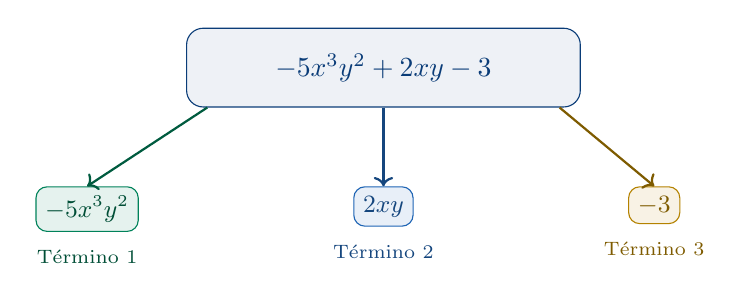
\begin{tikzpicture}[scale=0.9]
      \node[draw=azul,fill=azul!7,rounded corners=6pt,
            minimum width=5cm,minimum height=1cm,
            font=\normalsize\bfseries,text=azul] (ex) at (0,0)
            {$-5x^{3}y^{2}+2xy-3$};

      \coordinate (sw) at ([xshift=0.3cm]ex.south west);
      \coordinate (s)  at (ex.south);
      \coordinate (se) at ([xshift=-0.3cm]ex.south east);

      \node[draw=verde,fill=verde!10,rounded corners=4pt,
            font=\small\bfseries,text=verde!60!black,
            below left=1cm and 0.6cm of ex] (t1) {$-5x^{3}y^{2}$};
      \node[draw=azulm,fill=azulm!10,rounded corners=4pt,
            font=\small\bfseries,text=azulm!70!black,
            below=1cm of ex] (t2) {$2xy$};
      \node[draw=dorado,fill=dorado!10,rounded corners=4pt,
            font=\small\bfseries,text=dorado!70!black,
            below right=1cm and 0.6cm of ex] (t3) {$-3$};

      \draw[->,verde!70!black,thick]   (sw)--(t1.north);
      \draw[->,azulm!70!black,thick]   (s) --(t2.north);
      \draw[->,dorado!70!black,thick]  (se)--(t3.north);

      \node[below=3pt of t1,font=\scriptsize,text=verde!60!black]
        {T\'ermino 1};
      \node[below=3pt of t2,font=\scriptsize,text=azulm!70!black]
        {T\'ermino 2};
      \node[below=3pt of t3,font=\scriptsize,text=dorado!70!black]
        {T\'ermino 3};
    \end{tikzpicture}
  \end{columns}
\end{frame}

\begin{frame}{T\'erminos Semejantes}
  \begin{columns}[T]
    \column{0.48\textwidth}
    \begin{cdef}{T\'erminos semejantes}
      Dos o m\'as t\'erminos son \textbf{semejantes} si tienen
      \emph{exactamente la misma parte literal}.
    \end{cdef}
    \vspace{5pt}
    \renewcommand{\arraystretch}{1.4}
    \begin{tabular}{>{\bfseries}ll}
      \toprule
      & T\'erminos\\\midrule
      \textcolor{verde}{S\'i} & $3x^{2},\;-7x^{2},\;\tfrac{1}{2}x^{2}$\\
      \textcolor{verde}{S\'i} & $5xy^{2},\;-xy^{2}$\\
      \textcolor{red!70!black}{No} & $4x^{2},\;4x^{3}$ (exp.\ distinto)\\
      \textcolor{red!70!black}{No} & $3xy,\;3x^{2}y$ (exp.\ distinto)\\
      \bottomrule
    \end{tabular}

    \column{0.48\textwidth}
    \begin{cprop}{Reducci\'on de t\'erminos semejantes}
      Se suma/resta solo el coeficiente, manteniendo la parte literal:
      \[\alpha\,t+\beta\,t=(\alpha+\beta)\,t\]
    \end{cprop}
    \vspace{5pt}
    \begin{cejec}{Simplificaci\'on}
      \small
      \[5x^{2}-3x+7x^{2}+x-2\]
      \begin{align*}
        &=(5+7)x^{2}+(-3+1)x-2\\
        &=\boxed{12x^{2}-2x-2}
      \end{align*}
    \end{cejec}
  \end{columns}
\end{frame}

\begin{frame}{Grado de un Polinomio}
  \begin{columns}[T]
    \column{0.5\textwidth}
    \begin{cdef}{Grado de un t\'ermino}
      Suma de los exponentes de todas sus variables:
      \[\deg\!\bigl(c\,x_1^{a_1}\cdots x_k^{a_k}\bigr)
        =\textstyle\sum_{i=1}^{k}a_i\]
    \end{cdef}
    \vspace{5pt}
    \begin{block}{Ejemplos}
      \small
      \begin{itemize}
        \item $\deg(4x^{3}y^{2})=3+2=5$
        \item $\deg(7xy)=1+1=2$
        \item $\deg(-8)=0$ (constante)
      \end{itemize}
    \end{block}

    \column{0.46\textwidth}
    \begin{cdef}{Grado de un polinomio}
      Es el \textbf{mayor grado} entre todos sus t\'erminos.
    \end{cdef}
    \vspace{5pt}
    \begin{cejec}{Determinar el grado}
      \small
      $P(x,y)=3x^{4}-2x^{2}y^{3}+xy-5$\\[4pt]
      Grados: $4,\ 5,\ 2,\ 0$.\\[4pt]
      $\therefore$ $P$ tiene \textbf{grado 5}.
    \end{cejec}
    \vspace{5pt}
    \begin{calert}{Forma can\'onica}
      Un polinomio en $x$ est\'a en \textbf{forma can\'onica}
      cuando sus t\'erminos est\'an ordenados de mayor a menor grado.
    \end{calert}
  \end{columns}
\end{frame}

% ══════════════════════════════════════════════════════════════════
\section{Patrones y Relaciones Algebraicas}
% ══════════════════════════════════════════════════════════════════

\begin{frame}{Identidades Notables}
  \begin{columns}[T]
    \column{0.48\textwidth}
    \begin{cprop}{Cuadrado de una suma}
      $(a+b)^{2}=a^{2}+2ab+b^{2}$
    \end{cprop}\vspace{4pt}
    \begin{cprop}{Cuadrado de una diferencia}
      $(a-b)^{2}=a^{2}-2ab+b^{2}$
    \end{cprop}\vspace{4pt}
    \begin{cprop}{Diferencia de cuadrados}
      $(a+b)(a-b)=a^{2}-b^{2}$
    \end{cprop}\vspace{4pt}
    \begin{cprop}{Cubo de una suma}
      $(a+b)^{3}=a^{3}+3a^{2}b+3ab^{2}+b^{3}$
    \end{cprop}

    \column{0.48\textwidth}
    {\color{azul}\textbf{Verificaci\'on geom\'etrica: $(a+b)^{2}$}}
    \vspace{6pt}

    % Fixed tikz: use explicit numeric values instead of \a+\b
    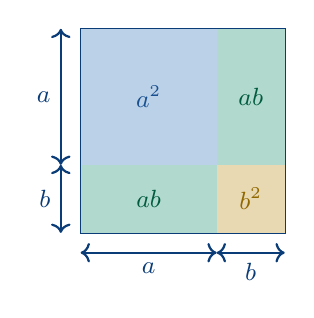
\begin{tikzpicture}[scale=0.72]
      % a=2.4, b=1.2, a+b=3.6
      \draw[thick,azul,fill=azul!5] (0,0) rectangle (3.6,3.6);
      \fill[azulm!30]  (0,1.2)   rectangle (2.4,3.6); % a^2
      \fill[dorado!30] (2.4,0)   rectangle (3.6,1.2); % b^2
      \fill[verde!30]  (0,0)     rectangle (2.4,1.2); % ab
      \fill[verde!30]  (2.4,1.2) rectangle (3.6,3.6); % ab

      \node[font=\small\bfseries,text=azulm!80!black]  at (1.2,2.4)  {$a^{2}$};
      \node[font=\small\bfseries,text=dorado!80!black] at (3.0,0.6)  {$b^{2}$};
      \node[font=\small,text=verde!70!black]           at (1.2,0.6)  {$ab$};
      \node[font=\small,text=verde!70!black]           at (3.0,2.4)  {$ab$};

      \draw[<->,thick,azul] (0,-0.35)--(2.4,-0.35)
        node[midway,below,font=\small]{$a$};
      \draw[<->,thick,azul] (2.4,-0.35)--(3.6,-0.35)
        node[midway,below,font=\small]{$b$};
      \draw[<->,thick,azul] (-0.35,0)--(-0.35,1.2)
        node[midway,left,font=\small]{$b$};
      \draw[<->,thick,azul] (-0.35,1.2)--(-0.35,3.6)
        node[midway,left,font=\small]{$a$};
    \end{tikzpicture}

    \vspace{4pt}
    \small
    ${\color{azul}(a+b)^{2}}=
     {\color{azulm!80!black}a^{2}}+
     {\color{verde!70!black}ab}+
     {\color{verde!70!black}ab}+
     {\color{dorado!80!black}b^{2}}$
  \end{columns}
\end{frame}

\begin{frame}{Tri\'angulo de Pascal y Binomio de Newton}
  \begin{columns}[T]
    \column{0.46\textwidth}
    {\color{azul}\textbf{Tri\'angulo de Pascal:}}
    \vspace{5pt}

    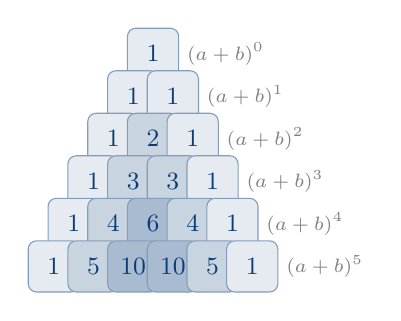
\begin{tikzpicture}[scale=0.72,
      nd/.style={draw=azul!50,fill=azul!10,rounded corners=3pt,
                 minimum size=0.65cm,font=\small,text=azul}]
      % Row 0
      \node[nd] at (0,0) {1};
      \node[font=\scriptsize\itshape,text=gray,right=2pt] at (0.33,0) {$(a+b)^0$};
      % Row 1
      \node[nd] at (-0.35,-0.75) {1};
      \node[nd] at ( 0.35,-0.75) {1};
      \node[font=\scriptsize\itshape,text=gray,right=2pt] at (0.68,-0.75) {$(a+b)^1$};
      % Row 2
      \node[nd] at (-0.70,-1.50) {1};
      \node[nd,fill=azul!22] at (0,-1.50) {2};
      \node[nd] at ( 0.70,-1.50) {1};
      \node[font=\scriptsize\itshape,text=gray,right=2pt] at (1.03,-1.50) {$(a+b)^2$};
      % Row 3
      \node[nd] at (-1.05,-2.25) {1};
      \node[nd,fill=azul!22] at (-0.35,-2.25) {3};
      \node[nd,fill=azul!22] at ( 0.35,-2.25) {3};
      \node[nd] at ( 1.05,-2.25) {1};
      \node[font=\scriptsize\itshape,text=gray,right=2pt] at (1.38,-2.25) {$(a+b)^3$};
      % Row 4
      \node[nd] at (-1.40,-3.00) {1};
      \node[nd,fill=azul!22] at (-0.70,-3.00) {4};
      \node[nd,fill=azul!35] at (0,-3.00) {6};
      \node[nd,fill=azul!22] at ( 0.70,-3.00) {4};
      \node[nd] at ( 1.40,-3.00) {1};
      \node[font=\scriptsize\itshape,text=gray,right=2pt] at (1.73,-3.00) {$(a+b)^4$};
      % Row 5
      \node[nd] at (-1.75,-3.75) {1};
      \node[nd,fill=azul!22] at (-1.05,-3.75) {5};
      \node[nd,fill=azul!35] at (-0.35,-3.75) {10};
      \node[nd,fill=azul!35] at ( 0.35,-3.75) {10};
      \node[nd,fill=azul!22] at ( 1.05,-3.75) {5};
      \node[nd] at ( 1.75,-3.75) {1};
      \node[font=\scriptsize\itshape,text=gray,right=2pt] at (2.08,-3.75) {$(a+b)^5$};
    \end{tikzpicture}

    \column{0.50\textwidth}
    \begin{cprop}{Teorema: Binomio de Newton}
      \[(a+b)^{n}=\sum_{k=0}^{n}\binom{n}{k}a^{n-k}b^{k}\]
      donde $\dbinom{n}{k}=\dfrac{n!}{k!(n-k)!}$
    \end{cprop}
    \vspace{5pt}
    \begin{cejec}{Expansi\'on de $(x-2)^{4}$}
      \small
      \begin{align*}
        &=\tbinom{4}{0}x^{4}(-2)^{0}
         +\tbinom{4}{1}x^{3}(-2)^{1}\\
        &\quad+\tbinom{4}{2}x^{2}(-2)^{2}
         +\tbinom{4}{3}x(-2)^{3}\\
        &\quad+\tbinom{4}{4}(-2)^{4}\\[4pt]
        &=\boxed{x^{4}-8x^{3}+24x^{2}-32x+16}
      \end{align*}
    \end{cejec}
  \end{columns}
\end{frame}

\begin{frame}{Inconsistencias: An\'alisis Cr\'itico}
  \begin{columns}[T]
    \column{0.5\textwidth}
    \begin{calert}{Inconsistencia 1: cancelaci\'on indebida}
      \small
      \textbf{Afirmaci\'on falsa:}
      \[\frac{x^{2}-4}{x-2}=x+2\quad\forall x\]
      \textbf{Error:} no definida para $x=2$.\\[4pt]
      \textbf{Correcto:}
      $\dfrac{x^{2}-4}{x-2}=x+2,\quad x\neq2$
    \end{calert}
    \vspace{5pt}
    \begin{calert}{Inconsistencia 2: potencia de suma}
      \small
      \textbf{Afirmaci\'on falsa:}
      $(3+5)^{2}\stackrel{?}{=}3^{2}+5^{2}=34$\\[4pt]
      \textbf{Correcto:} $(3+5)^{2}=64$\\
      Falta el t\'ermino cruzado $2\cdot3\cdot5=30$.
    \end{calert}

    \column{0.46\textwidth}
    \begin{block}{Estrategia: detecci\'on de errores}
      \small
      Para verificar una identidad algebraica aplica el
      \textbf{m\'etodo de sustituci\'on num\'erica}.\\[6pt]
      Si la igualdad falla para \emph{un} valor $\Rightarrow$
      es \textbf{falsa}.\\[6pt]
      Si se verifica para \emph{todos}, considerar demostraci\'on
      formal.
    \end{block}
    \vspace{5pt}
    \begin{cejec}{Detecta el error}
      \small
      \[\frac{a^{2}}{a}\stackrel{?}{=}a\quad\forall a\in\mathbb{R}\]
      \textit{?`Para qu\'e valores falla?}\\[4pt]
      \textbf{Respuesta:} Falla en $a=0$.\\
      V\'alido s\'olo para $a\neq0$.
    \end{cejec}
  \end{columns}
\end{frame}

\begin{frame}{Patrones en Sucesiones y Polinomios}
  \begin{columns}[T]
    \column{0.5\textwidth}
    \begin{block}{Sucesi\'on de cuadrados perfectos}
      \small
      $1,\ 4,\ 9,\ 16,\ 25,\ \ldots\quad a_{n}=n^{2}$\\[5pt]
      \textbf{Diferencias de 1er orden:}\ $3,5,7,9,\ldots$\\
      \textbf{Diferencias de 2do orden:}\ $2,2,2,\ldots$ (\emph{cte.})\\[5pt]
      Un polinomio de grado $k$ tiene diferencias finitas
      de orden $k$ \textbf{constantes}.
    \end{block}
    \vspace{5pt}
    \begin{cejec}{Identifica el grado}
      \small
      La sucesi\'on $1,8,27,64,125,\ldots$ corresponde a $n^{3}$.\\
      Verifica que sus diferencias de orden 3 son constantes.
    \end{cejec}

    \column{0.46\textwidth}
    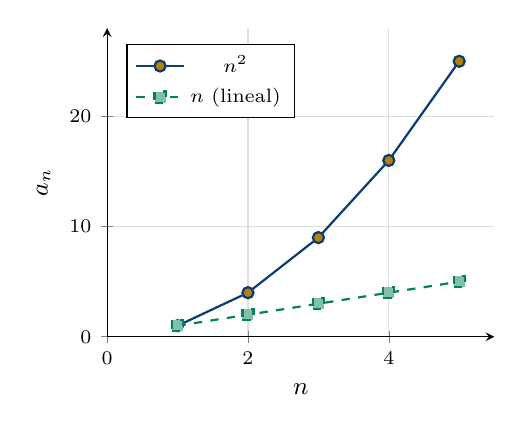
\begin{tikzpicture}
      \begin{axis}[
        width=6.5cm,height=5.5cm,
        xlabel={$n$},ylabel={$a_n$},
        xlabel style={font=\small},
        ylabel style={font=\small},
        tick label style={font=\scriptsize},
        grid=both,grid style={gray!25},
        axis lines=left,ymin=0,ymax=28,xmin=0,xmax=5.5,
        legend style={font=\scriptsize,at={(0.05,0.95)},anchor=north west}]
        \addplot[azul,thick,mark=*,mark options={fill=dorado}]
          coordinates{(1,1)(2,4)(3,9)(4,16)(5,25)};
        \addlegendentry{$n^2$}
        \addplot[verde,thick,dashed,mark=square*,mark options={fill=verde!50}]
          coordinates{(1,1)(2,2)(3,3)(4,4)(5,5)};
        \addlegendentry{$n$ (lineal)}
      \end{axis}
    \end{tikzpicture}
    \vspace{4pt}
    \begin{block}{Relaci\'on clave}
      \small El exponente determina la \textbf{tasa de crecimiento}:
      cuadr\'atico vs.\ lineal.
    \end{block}
  \end{columns}
\end{frame}

% ══════════════════════════════════════════════════════════════════
% EJERCICIOS INTEGRADORES
% ══════════════════════════════════════════════════════════════════

\begin{frame}{Ejercicios Integradores}
  \begin{columns}[T]
    \column{0.48\textwidth}
    \begin{cejec}{Nivel I --- Propiedades}
      \small Simplifica:
      \begin{enumerate}[a)]
        \item $\dfrac{(x^{2}y)^{3}\cdot x^{-1}}{x^{4}y^{2}}$
        \item $(2a^{3}b^{-2})^{2}\cdot(ab)^{-1}$
        \item $\dfrac{3^{n+2}-3^{n}}{3^{n}}$
      \end{enumerate}
    \end{cejec}
    \vspace{5pt}
    \begin{cejec}{Nivel II --- T\'erminos semejantes}
      \small Reduce y clasifica:
      \[(3x^{2}-2x+1)+(x^{2}+5x-4)-(x^{2}-x+2)\]
    \end{cejec}

    \column{0.48\textwidth}
    \begin{cejec}{Nivel III --- Identidades}
      \small
      \begin{enumerate}[a)]
        \item Expande: $(2x-3)^{2}+(2x+3)^{2}$
        \item Factoriza: $9a^{4}-24a^{2}b+16b^{2}$
        \item Demuestra:\\
          $(x+y)^{3}-(x-y)^{3}=2y(3x^{2}+y^{2})$
      \end{enumerate}
    \end{cejec}
    \vspace{5pt}
    \begin{cejec}{Nivel IV --- Patrones}
      \small
      Para $P(n)=2n^{2}-n+3$, calcula $P(1),\ldots,P(5)$,
      construye las diferencias finitas y verifica que son
      de orden~2.
    \end{cejec}
  \end{columns}
\end{frame}

% ══════════════════════════════════════════════════════════════════
% SINTESIS
% ══════════════════════════════════════════════════════════════════

\begin{frame}{S\'intesis de la Sesi\'on}
  \begin{columns}[T]
    \column{0.5\textwidth}
    \begin{block}{\checkmark\ Lo que aprendimos hoy}
      \small
      \begin{itemize}
        \item[\textcolor{verde}{$\checkmark$}]
          \textbf{Potencia} como producto iterado: $a^n$
        \item[\textcolor{verde}{$\checkmark$}]
          \textbf{Propiedades} P1--P5 y exponentes negativos
        \item[\textcolor{verde}{$\checkmark$}]
          \textbf{T\'ermino} y \textbf{expresi\'on algebraica}; grado
        \item[\textcolor{verde}{$\checkmark$}]
          \textbf{T\'erminos semejantes}: reducci\'on
        \item[\textcolor{verde}{$\checkmark$}]
          \textbf{Identidades notables} como patrones
        \item[\textcolor{verde}{$\checkmark$}]
          \textbf{Detecci\'on de inconsistencias} algebraicas
      \end{itemize}
    \end{block}

    \column{0.46\textwidth}
    \begin{block}{Mapa conceptual}
      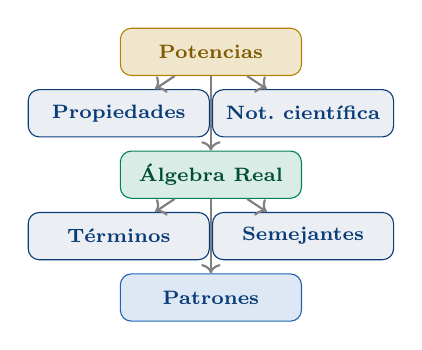
\begin{tikzpicture}[
        scale=0.78,
        box/.style={draw=azul,fill=azul!8,rounded corners=4pt,
                    font=\scriptsize\bfseries,text=azul,
                    minimum width=2.3cm,minimum height=0.6cm}]
        \node[box,fill=dorado!20,draw=dorado,text=dorado!70!black]
          (pot) at (0,0) {Potencias};
        \node[box] (prop) at (-1.5,-1.0) {Propiedades};
        \node[box] (notc) at ( 1.5,-1.0) {Not.\ cient\'ifica};
        \node[box,fill=verde!15,draw=verde,text=verde!60!black]
          (alg) at (0,-2.0) {\'Algebra Real};
        \node[box] (term) at (-1.5,-3.0) {T\'erminos};
        \node[box] (sem)  at ( 1.5,-3.0) {Semejantes};
        \node[box,fill=azulm!15,draw=azulm]
          (pat) at (0,-4.0) {Patrones};
        \draw[->,gray,thick] (pot)--(prop);
        \draw[->,gray,thick] (pot)--(notc);
        \draw[->,gray,thick] (pot)--(alg);
        \draw[->,gray,thick] (alg)--(term);
        \draw[->,gray,thick] (alg)--(sem);
        \draw[->,gray,thick] (alg)--(pat);
      \end{tikzpicture}
    \end{block}
  \end{columns}

  \vspace{7pt}
  \begin{center}
    \fcolorbox{dorado}{dorado!12}{%
      \parbox{0.88\textwidth}{\centering\small\itshape\color{dorado!70!black}
        ``El \'algebra es el lenguaje que usa la matem\'atica
        para revelar los patrones ocultos del universo.''}}
  \end{center}
\end{frame}

\begin{frame}{Tarea y Lecturas Complementarias}
  \begin{columns}[T]
    \column{0.5\textwidth}
    \begin{block}{\ding{46}\ Para la pr\'oxima sesi\'on}
      \small
      \begin{enumerate}
        \item Demostrar formalmente P3, P4 y P5 desde la definici\'on.
        \item Resolver los ejercicios integradores con procedimiento
              completo.
        \item Investigar la conexi\'on entre el Tri\'angulo de Pascal
              y las combinaciones $\binom{n}{k}$.
        \item Proponer una ``inconsistencia'' algebraica frecuente
              y su correcci\'on.
      \end{enumerate}
    \end{block}

    \column{0.46\textwidth}
    \begin{block}{Bibliograf\'ia}
      \small
      \begin{itemize}
        \item Stewart, J.\ (2018). \textit{Prec\'alculo}, 7.a ed.\
              Cengage.
        \item Apostol, T.\ (2006). \textit{Calculus}, vol.\ 1,
              2.a ed.\ Wiley.
        \item Lay, D.\ et al.\ (2016). \textit{\'Algebra Lineal},
              5.a ed.\ Pearson.
        \item Spivak, M.\ (2008). \textit{Calculus}, 4th ed.\
              Publish or Perish.
      \end{itemize}
    \end{block}
    \vspace{5pt}
    \begin{center}
      \large\textbf{\color{azul}?`Preguntas?}
    \end{center}
  \end{columns}
\end{frame}

\end{document}
